\section{Auf- und Entladen des Kondensatores über verschiedene Widerstände}

\begin{figure}[t]
    \centering
    \begin{minipage}[t]{0.32\linewidth}
        \centering
        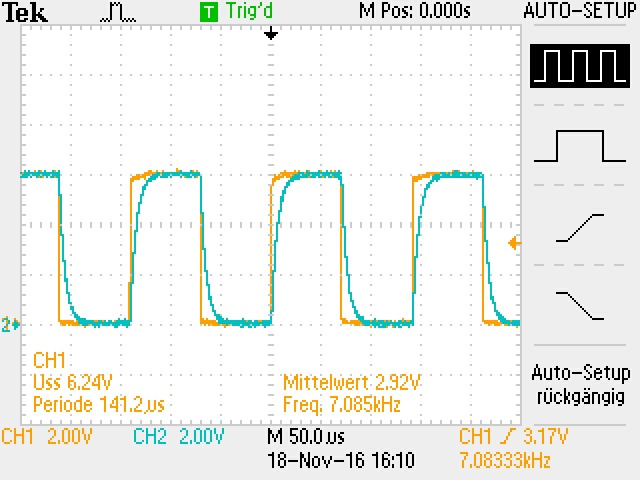
\includegraphics[width=\linewidth]{F0003TEK.jpg}
    \end{minipage}
    \begin{minipage}[t]{0.32\linewidth}
        \centering
        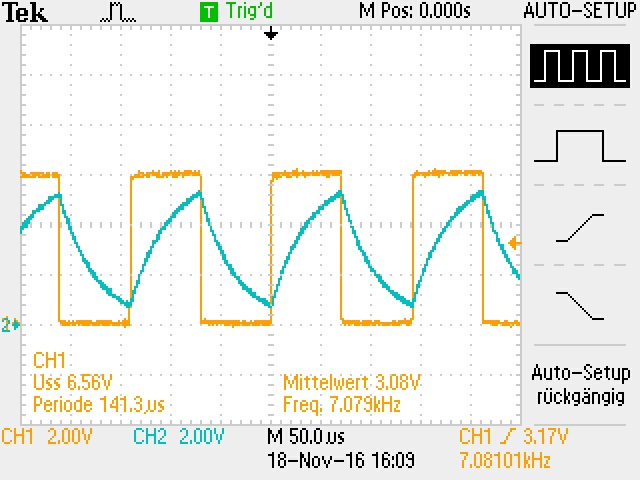
\includegraphics[width=\linewidth]{F0001TEK.jpg}
    \end{minipage}
    \begin{minipage}[t]{0.32\linewidth}
        \centering
        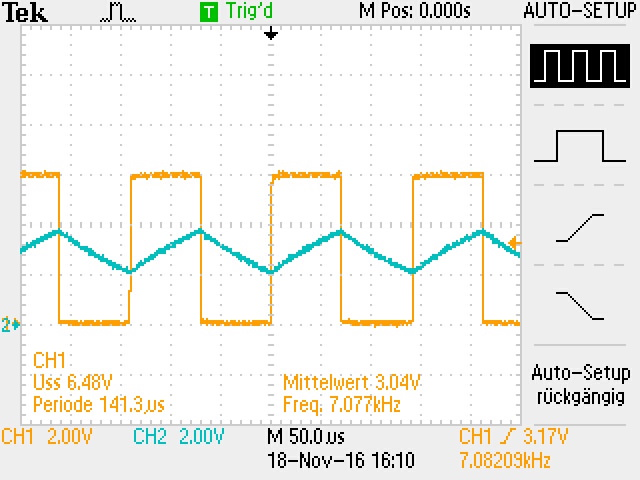
\includegraphics[width=\linewidth]{F0002TEK.jpg}
    \end{minipage}
    \caption*{Bild 1:\small Spannung am Kondenstator aufgetragen gegen die Zeit (Blau), bei anliegender Rechteckspannung (Orange) und für von links nach rechts größer werdenden Widerstand}
\end{figure}


Wie in Bild 1 zu sehen ist steigt und sinkt die Spannung am Kondensator für einen größeren Widerstand langsamer. Da die Spannung an einem Kondensator proportional zu der Ladungsdifferenz zwischen den beiden Kondensatorplatten ist, bedeutet das, dass bei einem größeren Widerstand sich die Kondensatorplatten
langsamer mit elektrische Ladung auf- und entladen. Wenn also die Platten sich langsamer auf- und entladen heißt das, dass weniger elektrische Ladung pro Zeit, also Strom, auf die Platten fließt. Den Zusammenhang, dass weniger Strom ($I$) fließt bei einem größeren Widerstand ($R$) sieht man an dem  Ohm`schen Gestz:
\begin{align}
    U=R\cdot I \text{\hspace{0.5cm},}
\end{align}
wobei U die Spannung am Widerstand ($R$) ist.

Man erkennt das Verhalten der Spannung am Kondensator für verschiedenewiderstände auch an der Formel:
\begin{align}
    U_C(t)=U_0 \left( 1-e^{-\frac{t}{\tau}} \right)\text{\hspace{0.5cm},}
\end{align}
wobei $U_C(t)$ die zeitlich abhängige Spannung am Kondensator ist, $U_0$ die Spannung an Kondensator und Widerstand und $\tau=RC$, mit $R$ dem Widerstand und $C$ der Kapazität des Kondensators. $\tau$ hat die Einheit Zeit und gibt an nach welcher Zeit die Spannung am Kondensator $\left(1-\frac{1}{e}\right)\,U_0\approx0,63\,U_0$ beträgt. Wird $\tau$ also größer, dann dauert es länger bis die Spannung am Kondensator $0,63\,U_0$ erreicht. Da gilt $\tau=RC$ wird $\tau$ also größer wenn $R$ größer wird. Somit läd und entläd sich der Kondensator mit größerem Widerstand $R$ langsamer.

\section{Bestimmung der Kapazität des Kondensators}
Um die Kapazität des Kondensators zu bestimmen wird zunächst der vom Oszilloskop erstellte Kurvenverlauf (Bild 2) auf Millimeterpapier übertragen. Dazu wurden die Messpunkte in Tabelle 1 aus der blauen Kurve in Bild 2 abgelesen. Die Fehler des Messwerte ergeben sich dadurch, dass aufgrund der dicke der Kurve und der etwas schlechten Auslösung des Bildes eine genaure Bestimmung nicht möglich war. Der auf Millimeterpapier übertragene Kurvenverlauf ist im Anhang zu finden.
\begin{figure}[h]
    \centering
    \begin{minipage}[h]{0.45\linewidth}
        \centering
        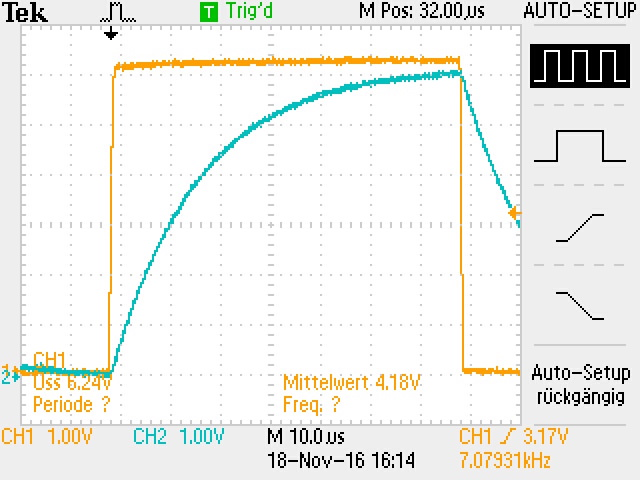
\includegraphics[width=\linewidth]{F0005TEK.jpg}
        \caption*{Bild 2: \small Aufladevorgang des Kondensators}
    \end{minipage}
    \hspace{0.2cm}
    \begin{minipage}[h]{0.45\linewidth}
        \centering
        \begin{tabular}{|c|c|c|}
            \hline
            Messwert& $t_i$ in $\mu s$ & $U_C(t_i)$ in V \\
            \hline
            \hline
            1 & 2 & $0,7\pm0,1$ \\
            \hline
            2 & 7 & $2,0\pm0,1$ \\
            \hline
            3 & 12 & $3,1\pm0,1$ \\
            \hline
            4 & 22 & $4,4\pm0,1$ \\
            \hline
            5 & 32 & $5,2\pm0,1$ \\
            \hline
            6 & 42 & $5,6\pm0,1$ \\
            \hline
            7 & 52 & $5,9\pm0,1$ \\
            \hline
            8 & 62 & $6,0\pm0,1$ \\
            \hline
        \end{tabular}
        \caption*{Tabelle 1: \small Aus Bild 2 bestimmte Messwerte}
    \end{minipage}
\end{figure}

Für die Spannung am Kondensator bei dem Aufladevorgang gilt die schon zuvor erwähnte Gleichung (2). Stellt man diese um, so gilt:
\begin{align}
    &&U_C(t) =&U_0 \left( 1-e^{-\frac{t}{\tau}} \right) && |:U_0\nonumber \\
    \Leftrightarrow &&\frac{U_C(t)}{U_0} =& 1-e^{-\frac{t}{\tau}} && |-1 \nonumber \\
    \Leftrightarrow &&\frac{U_C(t)}{U_0} -1 =& -e^{-\frac{t}{\tau}} && |\cdot(-1)\nonumber \\
    \Leftrightarrow && 1-\frac{U_C(t)}{U_0} =& e^{-\frac{t}{\tau}} && |\ln()\nonumber \\
    \Leftrightarrow && \ln\left(1-\frac{U_C(t)}{U_0}\right) =& -\frac{1}{\tau} \cdot t \hspace{1cm}.
\end{align}
Es werden nun für die Messwerte aus der Tabelle 1 $\ln\left(1-\frac{U_C(t_i)}{U_0}\right)$ berechnet, wobei $U_0$ die in der Durchführung gemessene Spannung der Rechteckspannung ist. Sie beträgt $U_0=(6,2 \pm 0,2)\,V$. Der Fehler für $\ln\left(1-\frac{U_C(t_i)}{U_0}\right)$ ergibt sich durch die Gaußsche Fehlerfortpflanzung von den Fehlern von $U_0$ und $U_C(t_i)$. Es gilt:
\begin{align*}
    \sigma_{\ln\left(1-\frac{U_C(t_i)}{U_0}\right)}
&=\sqrt{\sigma_{U_0}^2 \left(\frac{\partial \ln\left(1-\frac{U_C(t_i)}{U_0}\right)}{\partial U_0}\right)^2 + \sigma_{U_C(t_i)}^2 \left(\frac{\partial \ln\left(1-\frac{U_C(t_i)}{U_0}\right)}{\partial U_C(t_i)}\right)^2 }\\
&=\sqrt{\sigma_{U_0}^2 \left(\frac{-\frac{U_C(t_i)}{U_0^2}}{\left(1-\frac{U_C(t_i)}{U_0}\right)}\right)^2 + \sigma_{U_C(t_i)}^2 \left(\frac{-\frac{1}{U_0}}{\left(1-\frac{U_C(t_i)}{U_0}\right)}\right)^2 }\\
&=\sqrt{ \left(\frac{\sigma_{U_0}\cdot U_C(t_i)}{\left(U_0^2-U_C(t_i) \cdot U_0\right)}\right)^2 +  \left(\frac{\sigma_{U_C(t_i)}}{\left(U_0-U_C(t_i)\right)}\right)^2 }\hspace{0.5cm},
\end{align*}
wobei $\sigma_{U_0}=0,2\,V$ der Fehler von $U_0$ ist und $\sigma_{U_C(t_1)}=0,1\,V$ der Fehler von den einzelnen Messwerten $U_C(t_i)$ ist. In Tabelle 2 wurden die Werte von $\ln\left(1-\frac{U_C(t_i)}{U_0}\right)$ mit den Fehlern notiert. Diese Werte sind gegen die Zeit aufgetragen wurden (siehe Anhang).
    \begin{table}[t]
        \centering
        \begin{tabular}{|c|c|c|}
            \hline
            Messwert& $t_i$ in $\mu s$ & $\ln\left(1-\frac{U_C(t_i)}{U_0}\right)$\\
            \hline
            \hline
            1 & 2 & $-0,12\pm0,02$ \\
            \hline
            2 & 7 & $-0,39\pm0,03$ \\
            \hline
            3 & 12 & $-0,70\pm0,05$ \\
            \hline
            4 & 22 & $-1,2\pm0,1$ \\
            \hline
            5 & 32 & $-1,8\pm0,2$ \\
            \hline
            6 & 42 & $-2,3\pm0,4$ \\
            \hline
            7 & 52 & $-3,0\pm0,8$ \\
            \hline
            8 & 62 & $-3,4\pm1,1$ \\
            \hline
        \end{tabular}
        \caption*{Tabelle 2: \small Werte für $\ln\left(1-\frac{U_C(t_i)}{U_0}\right)$}
    \end{table} 
Es ist ein linearer Zusammenhang zwischen der Zeit und $\ln\left(1-\frac{U_C(t_i)}{U_0}\right)$ ersichtlich. Für die Gerade dieses Zusammenhanges wurde die Steigung $m$ mit $m=(-60\pm20)\,$kHz bestimmt. Aus Gleichung (3) ist zu erkennen, dass diese Steigung dem Faktor vor dem $t$ entsprechen muss. Also:
\begin{align}
   && m&=-\frac{1}{\tau} && |\tau=RC \nonumber\\
   \Leftrightarrow && m&= -\frac{1}{RC} && |\cdot R \nonumber\\
   \Leftrightarrow && mR&= -\frac{1}{C} && |\cdot (-1) \nonumber\\
   \Leftrightarrow && -mR&= \frac{1}{C} && |\frac{1}{()} \nonumber\\
   \Leftrightarrow &&  -\frac{1}{mR}  &= C &&.
\end{align}
Somit haben wir eine Gleichung für die Kapazität des Kondensators. Dabei ist $m$ die bestimmt Steigung und $R=R_C=(2,48\pm0,03)\,k\Omega$ der im Versuch gemessene Widerstand vor dem Kondensator. Der Fehler von $C$ ergibt sich durch die Gaußsche Fehlerfortpflanzung der Fehler von $m$ und $R$. Es gilt:
\begin{align}
    \sigma_{C}&=\sqrt{\sigma_{m}^2 \left(\frac{\partial C}{\partial m}\right)^2 + \sigma_{R}^2 \left(\frac{\partial C}{\partial R}\right)^2 } = \sqrt{\sigma_{m}^2 \left(-\frac{1}{m^2R}\right)^2 + \sigma_{R}^2 \left(-\frac{1}{mR^2}\right)^2 }\nonumber\\
    &=\left|\frac{1}{mR}\right|\sqrt{ \left(\frac{\sigma_{m}}{m}\right)^2 +  \left(\frac{\sigma_{R}}{R}\right)^2 }\hspace{0,5cm},
\end{align}
mit $\sigma_m=20\,$kHz und $\sigma_R=0,03\,k\Omega$. Mit Gleichung (4) ergibt sich der Wert von $C$ und mit Gleichung (5) der entsprechende Fehler von $C$. Somit ist die Kapazität des Kondensators:
\begin{align*}
  \underline{\underline{C=(7\pm3)\cdot 10^{-9}\,\frac{1}{\text{Hz}\cdot\Omega}=(7\pm3)\,\text{nF}}}.
\end{align*}
\newpage
\section{R-L-Kreis als Hochpassfilter}
\begin{figure}[!htb]
    \centering
    \begin{minipage}[t]{0.7\linewidth}
        \centering
        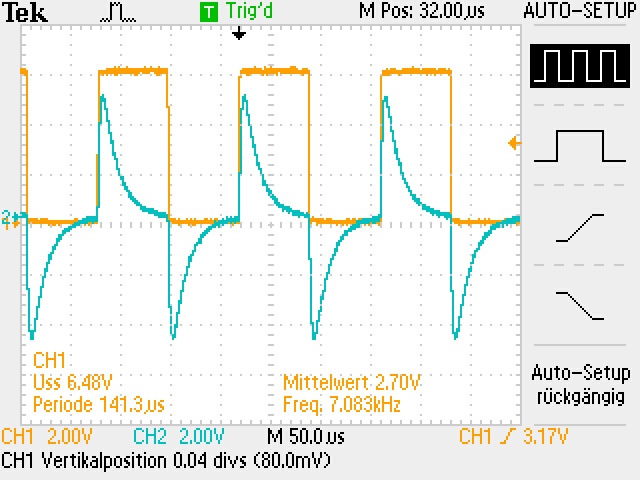
\includegraphics[width=\linewidth]{F0006TEK.jpg}
    \end{minipage}
    \caption*{Bild 3: \small Spannung an der Spule aufgetragen gegen die Zeit (Blau) bei anliegender Rechteckspannung (Orange)}
\end{figure}
Wie in Bild 3 zu sehen ist setzt die Spannung an der Spule anfangs zusammen mit der Spannung an Widerstand und Spule plötzlich ein, doch während die Spannung an Widerstand und Spule (Orange) dort bleibt sinkt die Spannung an der Spule (Blau) exponentiell. Also wenn sich die Spannung an Widerstand und Spule nicht ändert so bildet die Spule einen Kurzschluss und es liegt keine Spannung mehr an ihr an. Wenn sich aber die Spannung schnell ändert so liegt annährend die selbe Spannung an der Spule an wie an dem Widerstand und Spule. Also bildet die Spule bei langsamen Änderungen der Spannung, also tiefen Frequenzen einen Kurzschluss und es liegt kaum Spannung an der Spule an und bei schnellen Änderungen der Spannung, also hohen Frequenzen, liegt an der Spule fast die selbe Spannung an und die Frequenz kommt durch. Aus diesem Grund nennt man den R-L-Kreis auch Hochpass, weil hohe Frequenzen passieren können und tiefe Frequenzen nicht.
\end{document}
